\documentclass{beamer}
\mode<presentation>
{
  \usetheme{Warsaw}
  \definecolor{mcgarnet}{rgb}{0.38, 0, 0.08}
  \definecolor{mcgray}{rgb}{0.6, 0.6, 0.6}
  \setbeamercolor{structure}{fg=mcgarnet,bg=mcgray}
  %\setbeamercovered{transparent}
}


\usepackage[english]{babel}
\usepackage[latin1]{inputenc}
\usepackage{times}
\usepackage[T1]{fontenc}
\usepackage{tikz}
\usepackage{graphicx}

\newcommand{\imagesource}[1]{{\centering\hfill\break\hbox{\scriptsize Image Source:\thinspace{\small\itshape #1}}\par}}

\title{HabPi: A Simple Framework for High Altitude Sensing}


\author{Robert Lowe\\}

\institute[Maryville College] % (optional, but mostly needed)
{
  Division of Mathematics and Computer Science\\
  Maryville College
}

\date[]{October 27, 2017}
\subject{}

\pgfdeclareimage[height=0.5cm]{university-logo}{images/Maryville-College}
\logo{\pgfuseimage{university-logo}}



\AtBeginSection[]
{
  \begin{frame}<beamer>{Outline}
    \tableofcontents[currentsection]
  \end{frame}
}


\begin{document}

\begin{frame}
  \titlepage
\end{frame}

\begin{frame}{Outline}
  \tableofcontents
\end{frame}


% Structuring a talk is a difficult task and the following structure
% may not be suitable. Here are some rules that apply for this
% solution: 

% - Exactly two or three sections (other than the summary).
% - At *most* three subsections per section.
% - Talk about 30s to 2min per frame. So there should be between about
%   15 and 30 frames, all told.

% - A conference audience is likely to know very little of what you
%   are going to talk about. So *simplify*!
% - In a 20min talk, getting the main ideas across is hard
%   enough. Leave out details, even if it means being less precise than
%   you think necessary.
% - If you omit details that are vital to the proof/implementation,
%   just say so once. Everybody will be happy with that.
\section{Introduction}

\section{HabPi}

\section{HabPi Flights}
\begin{frame}{HabPi 1 - November 18, 2016}
    \begin{itemize}[<+->]
        \item The first unteathered flight of the PSCC/MC Balloon
          Team
        \item HabPi payload was constructed by the students of
        Maryville College
        \item Released from PSCC Hardin Valley Campus in Knoxville, TN
        \item Reached an altitude of approximately 30,000 meters
        \item Came to rest in Pisgah National Forest near Blowing
           Rock, NC
    \end{itemize}
\end{frame}
\begin{frame}{HabPi 1 - November 18, 2016}
    \begin{figure}
        \centering
        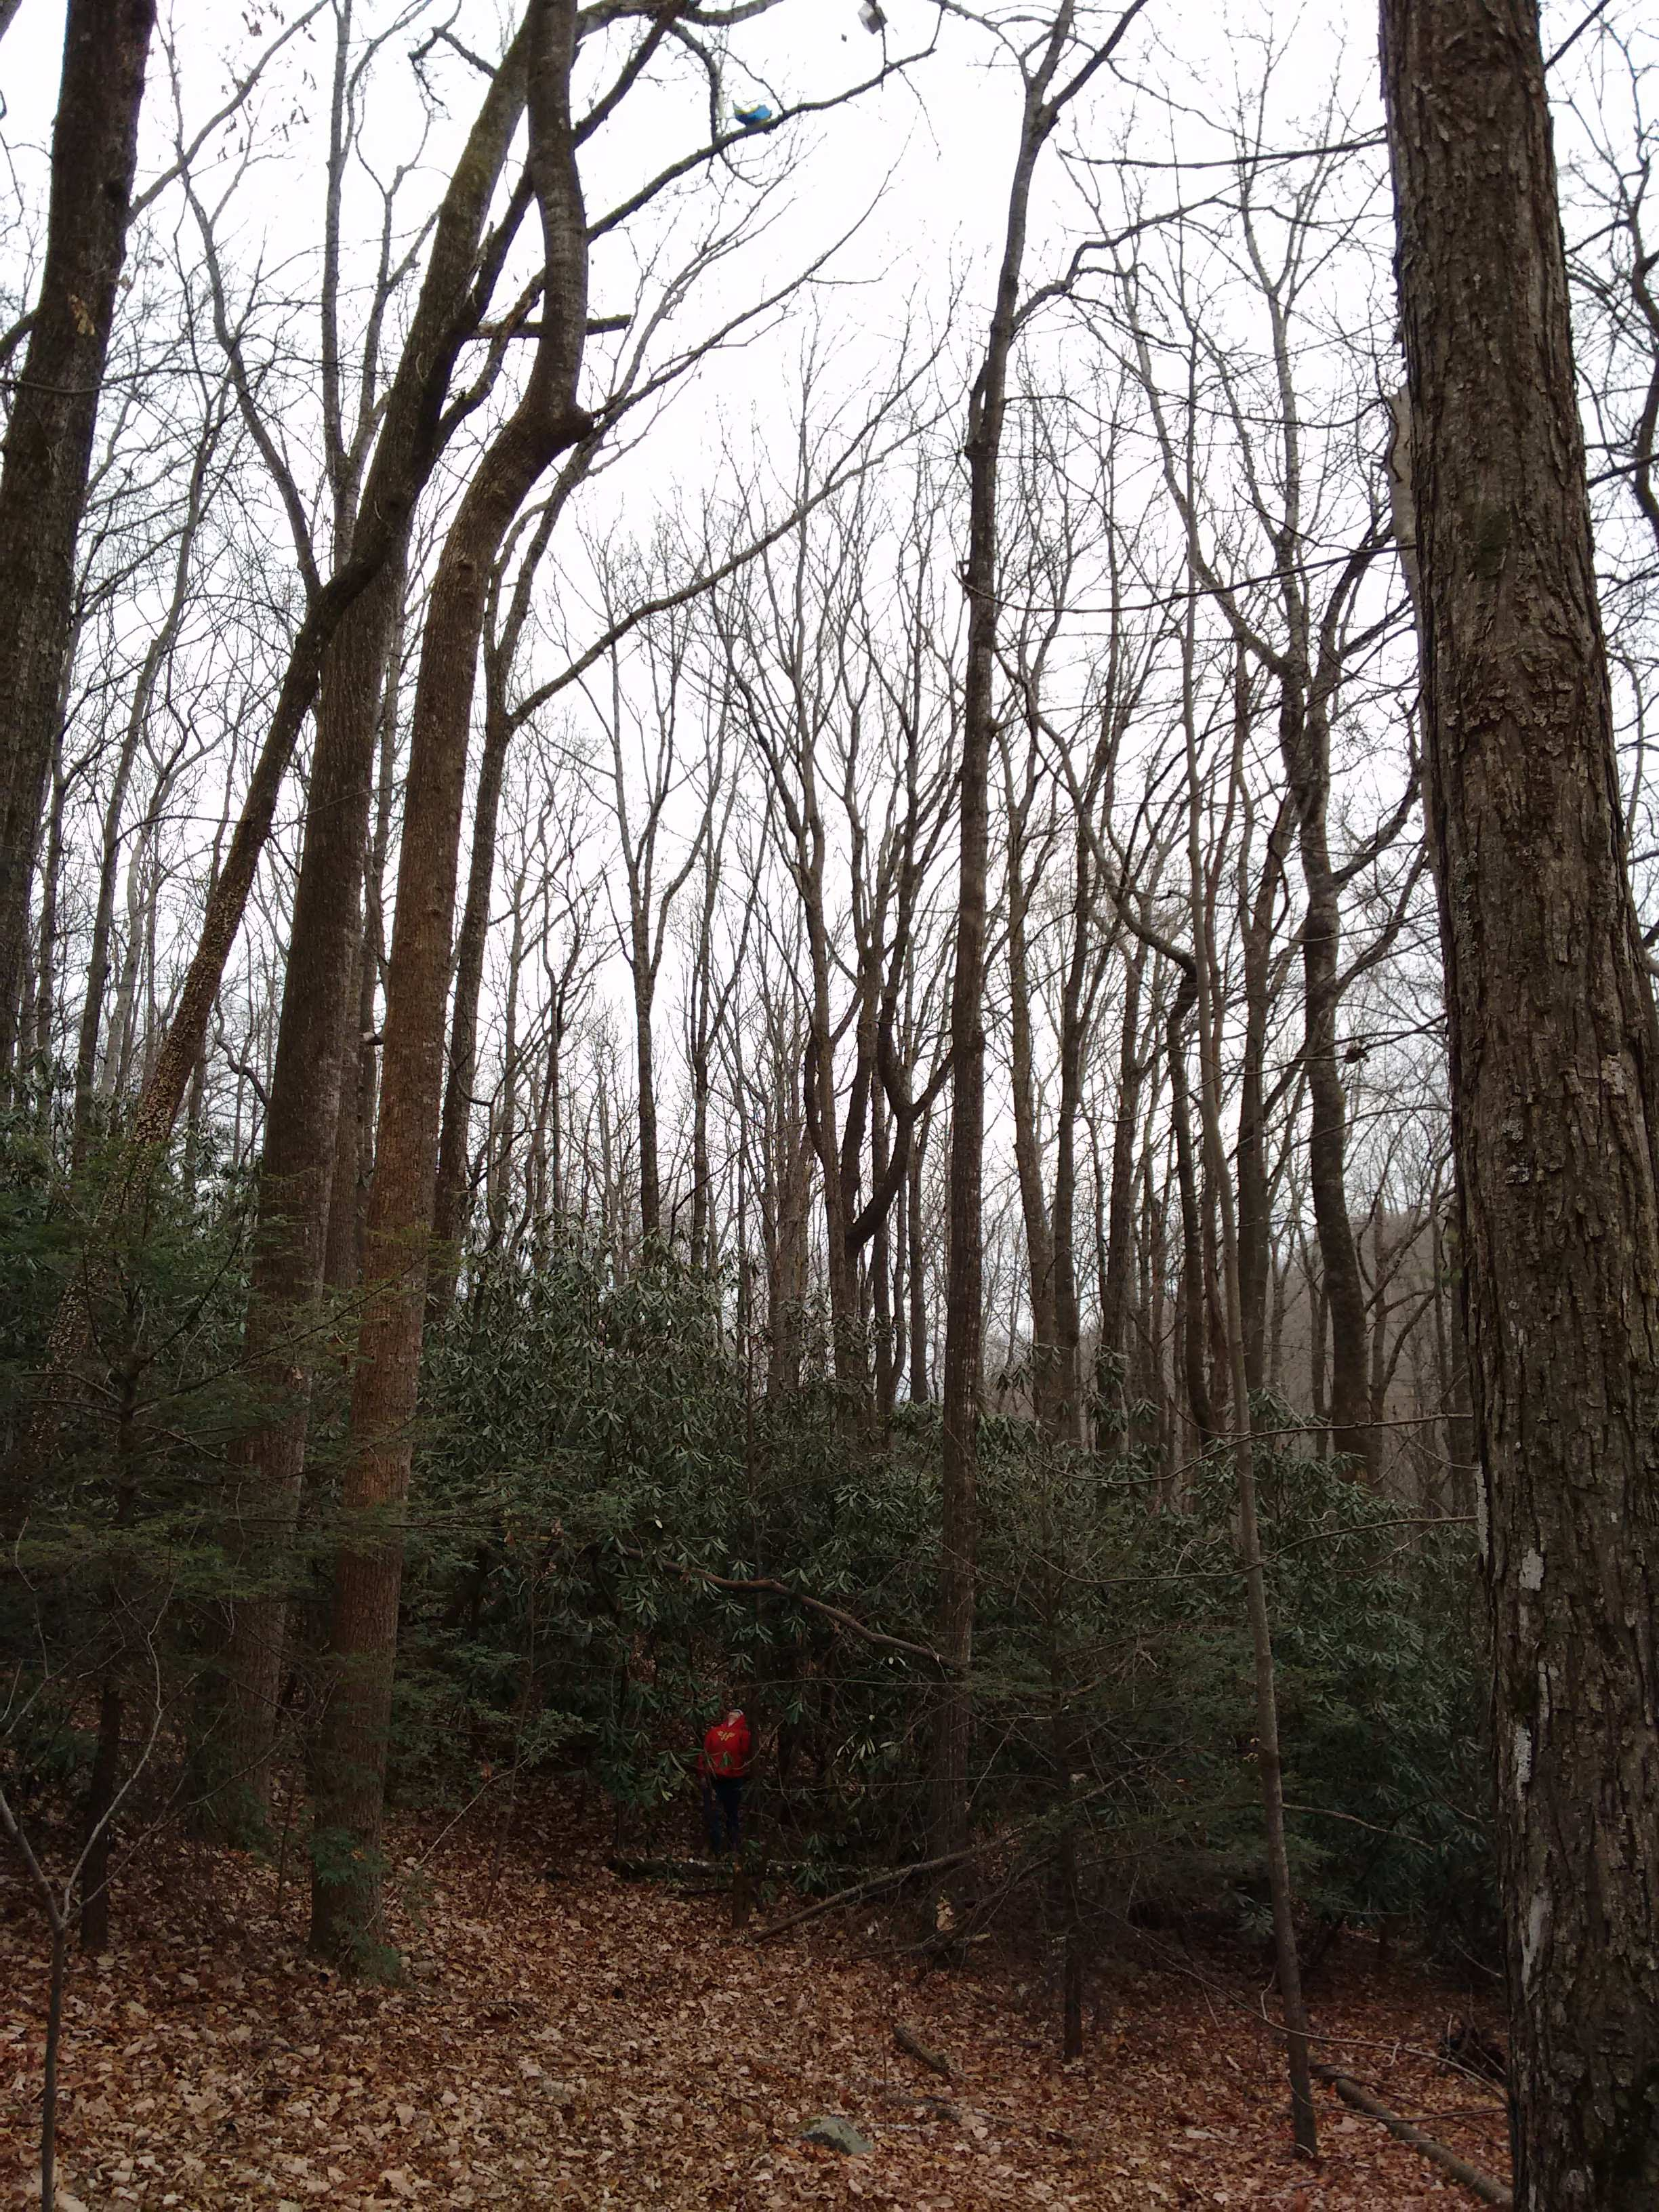
\includegraphics[height=0.75\textheight]{images/HabPi1_1}
        \caption{HabPi 1 in Tree}
    \end{figure}
\end{frame}

\begin{frame}[t]{HabPi 2 - March 19, 2017}
    \begin{columns}[t]
        \column{0.5\textwidth}
        \begin{itemize}
            \item Reference HabPi device built by Robert Lowe
            \item Released from Russell Springs Kentucky
            \item Reached an Altitude of 42,000 Meters
            \item Recovered near New River, TN
        \end{itemize}

        \column{0.5\textwidth}
        \begin{figure}
            \centering
            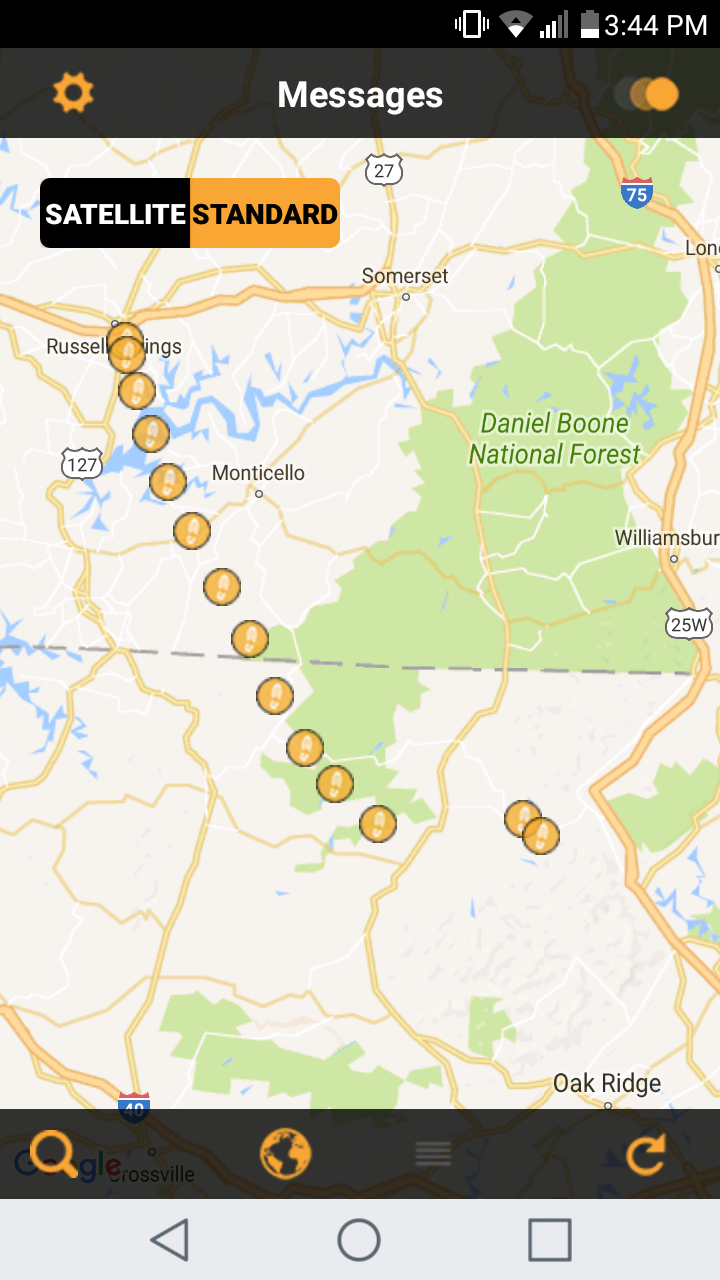
\includegraphics[height=0.6\textheight]{images/habpi2_track}
            \caption{\tiny HabPi 2 Spot Tracker}
        \end{figure}
    \end{columns}
\end{frame}

\begin{frame}{HabPi 2 - March 19, 2017}
    \begin{figure}
        \centering
        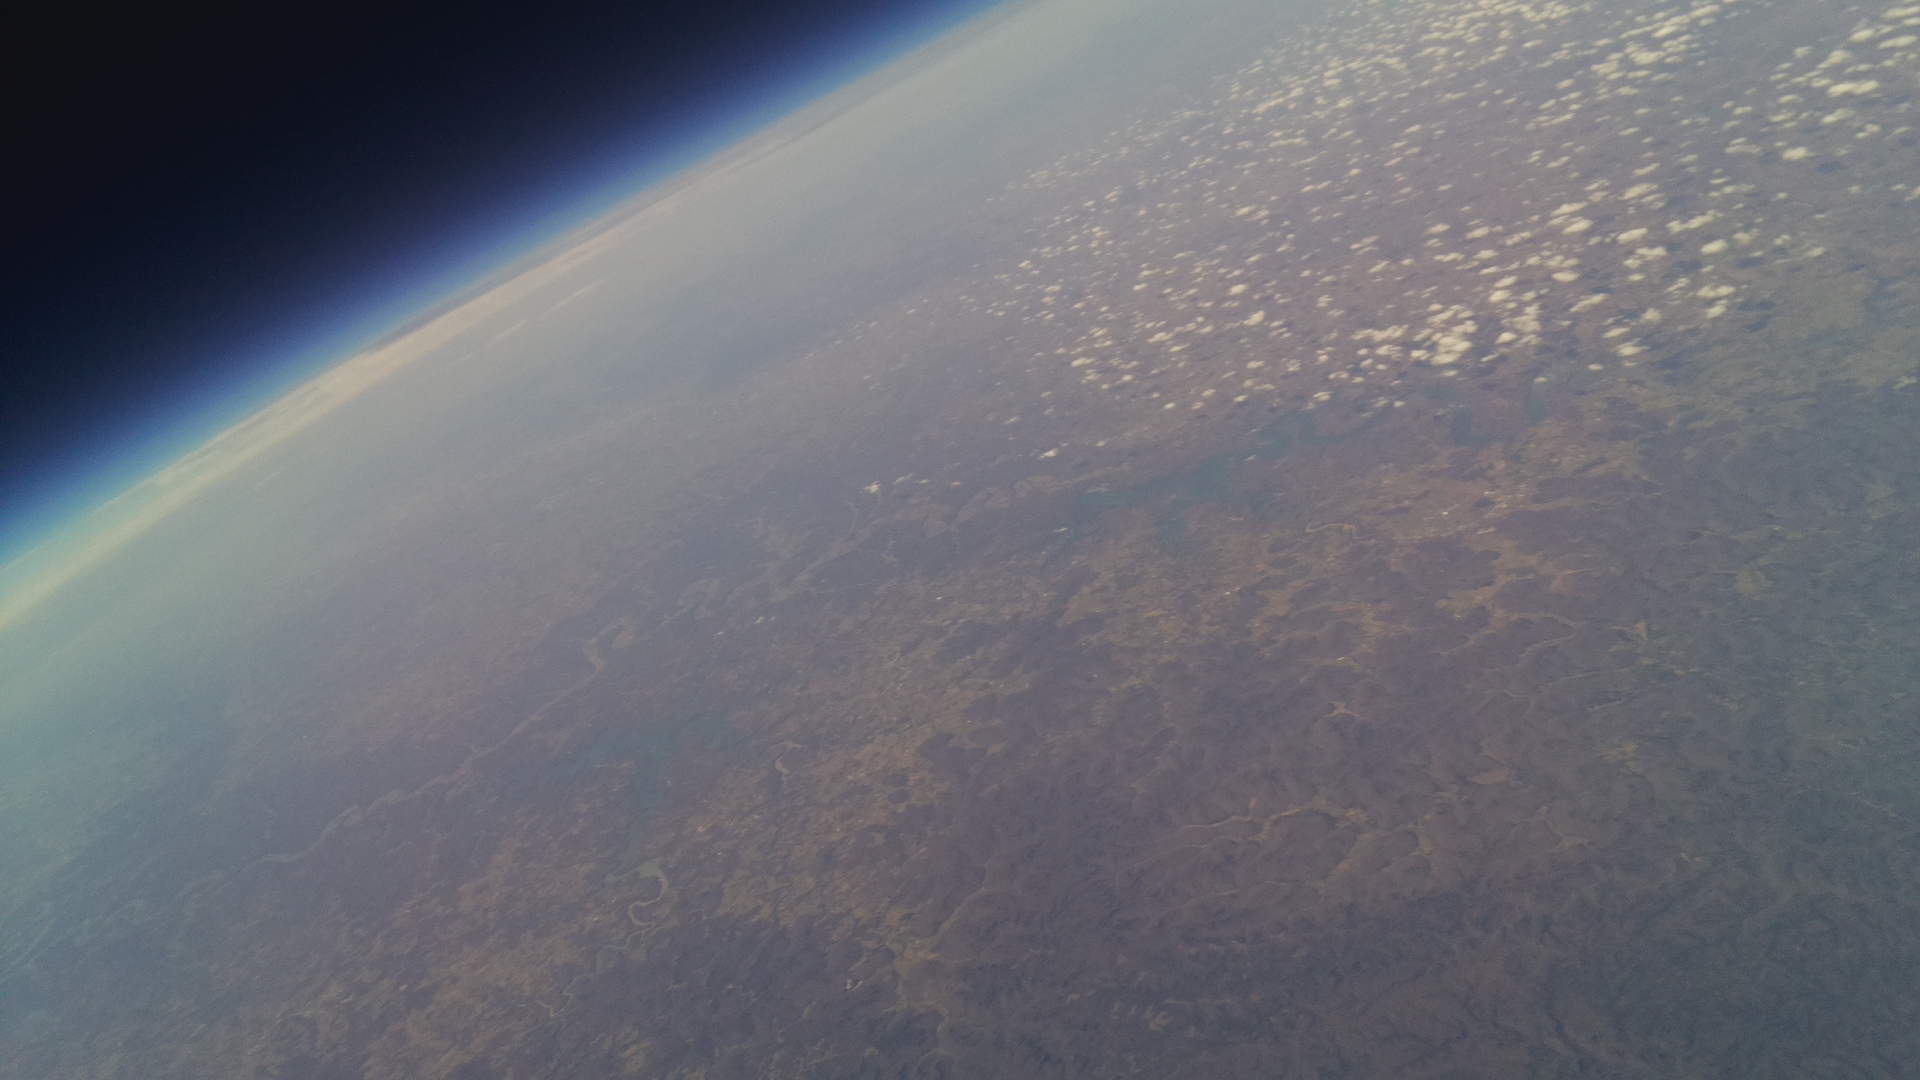
\includegraphics[width=\textwidth]{images/habpi2_1}
    \end{figure}
\end{frame}

\begin{frame}{HabPi 2 - March 19, 2017}
    \begin{figure}
        \centering
        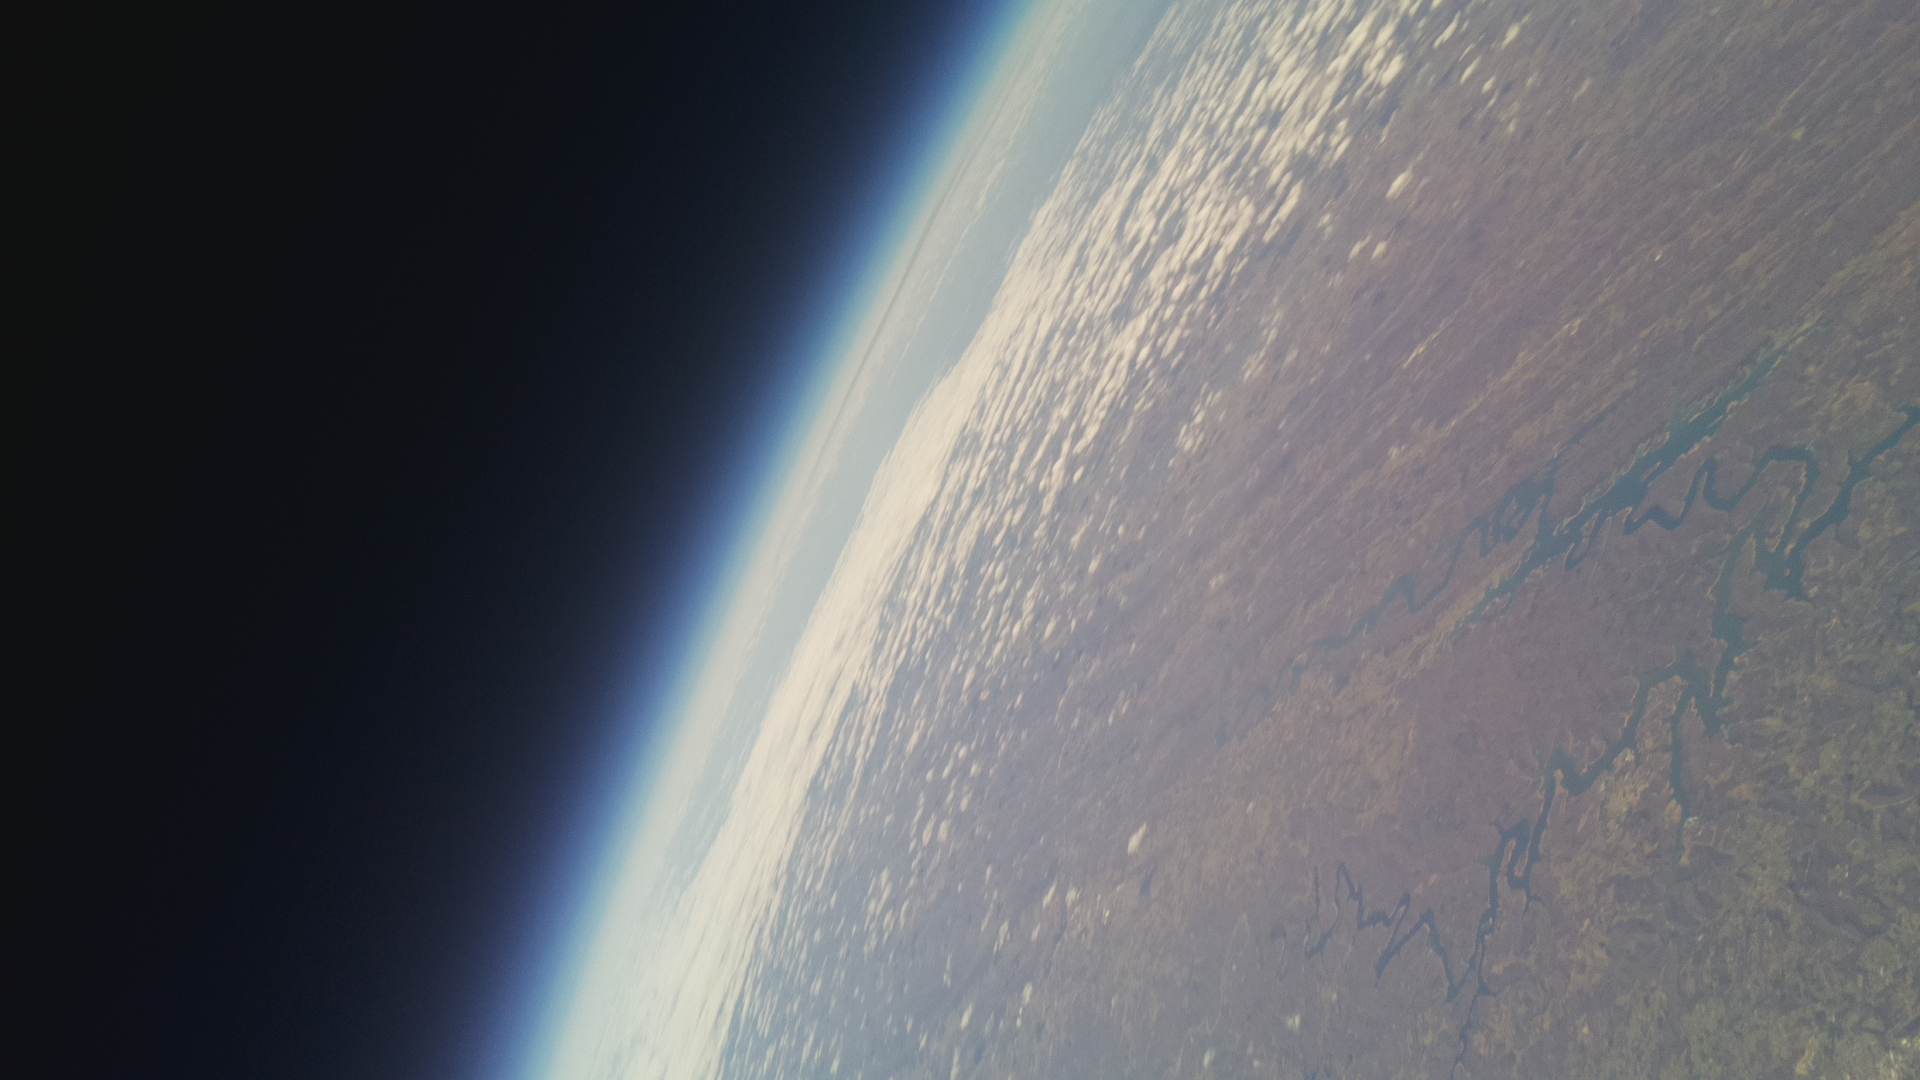
\includegraphics[width=\textwidth]{images/habpi2_2}
    \end{figure}
\end{frame}

\begin{frame}{HabPi 2 - March 19, 2017}
    \begin{figure}
        \centering
        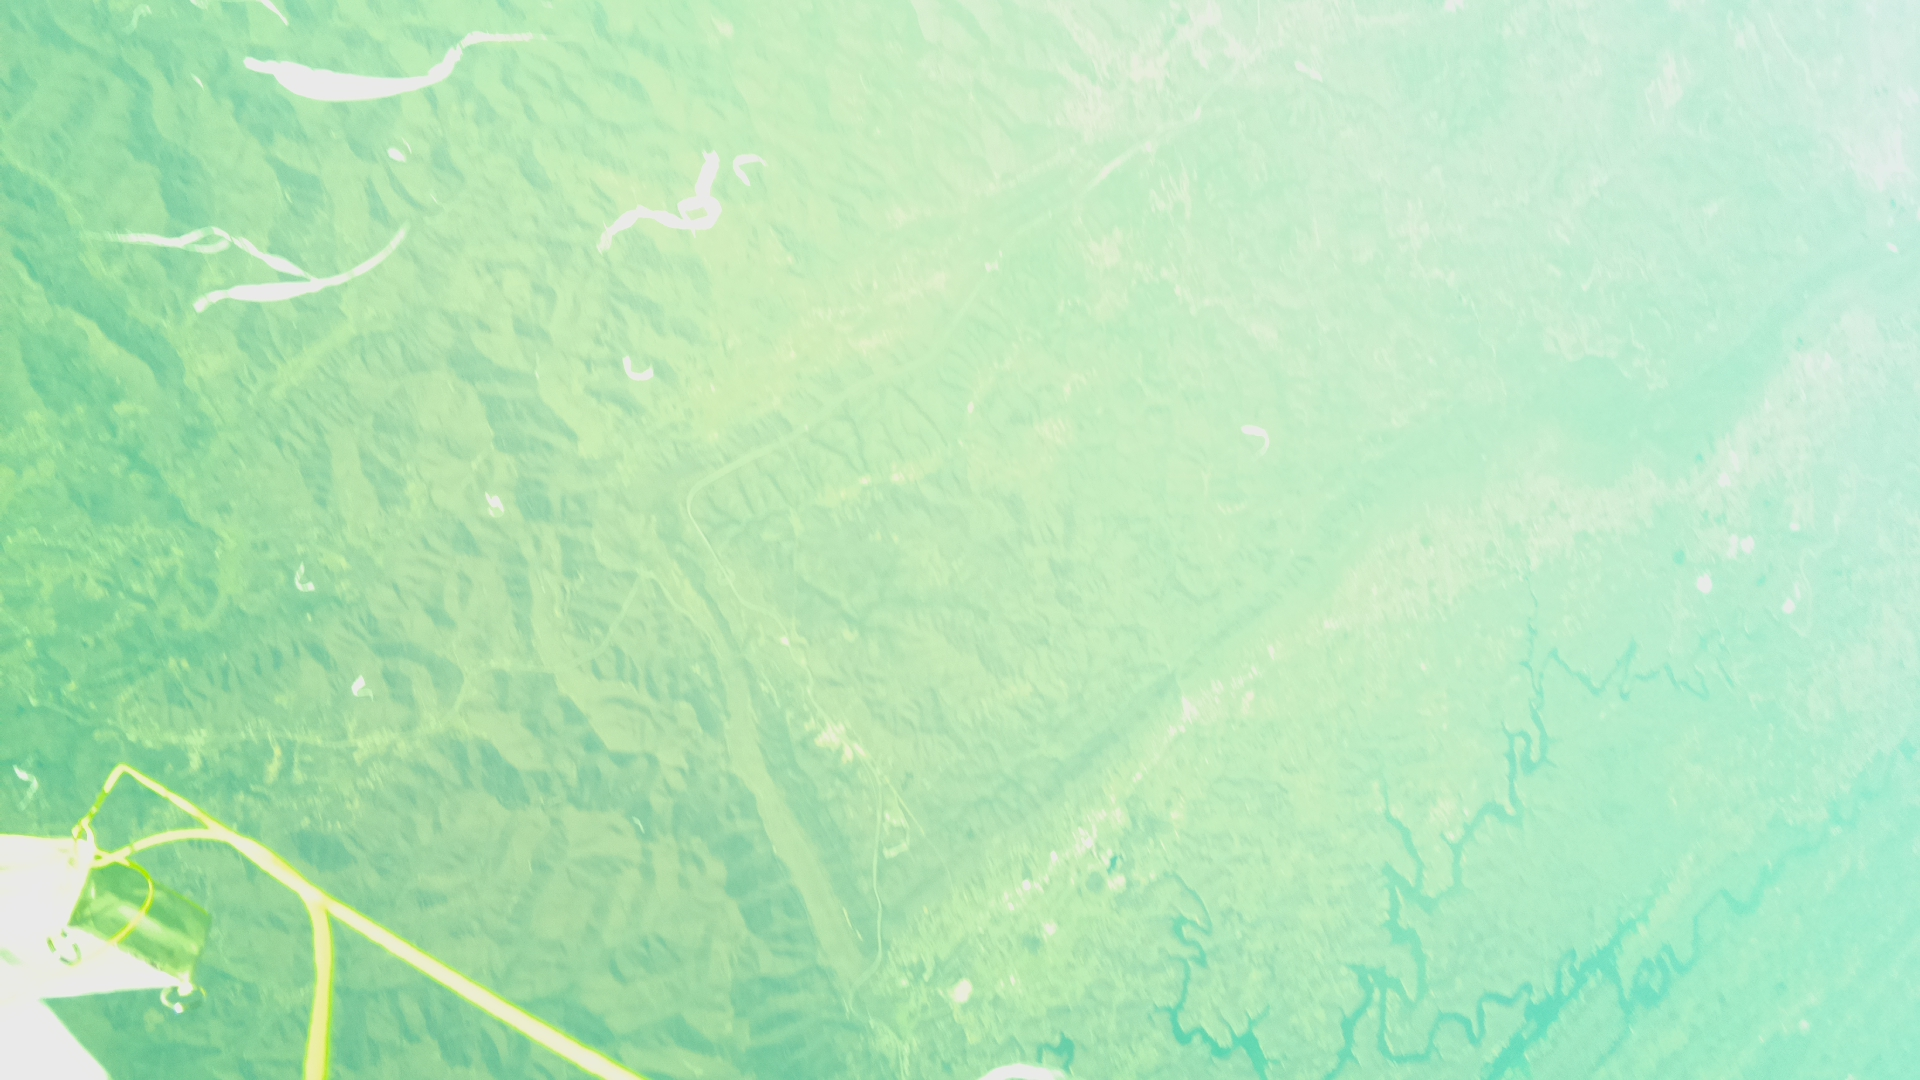
\includegraphics[width=\textwidth]{images/habpi2_3}
    \end{figure}
\end{frame}

\begin{frame}{HabPi 2 - March 19, 2017}
    \begin{figure}
        \centering
        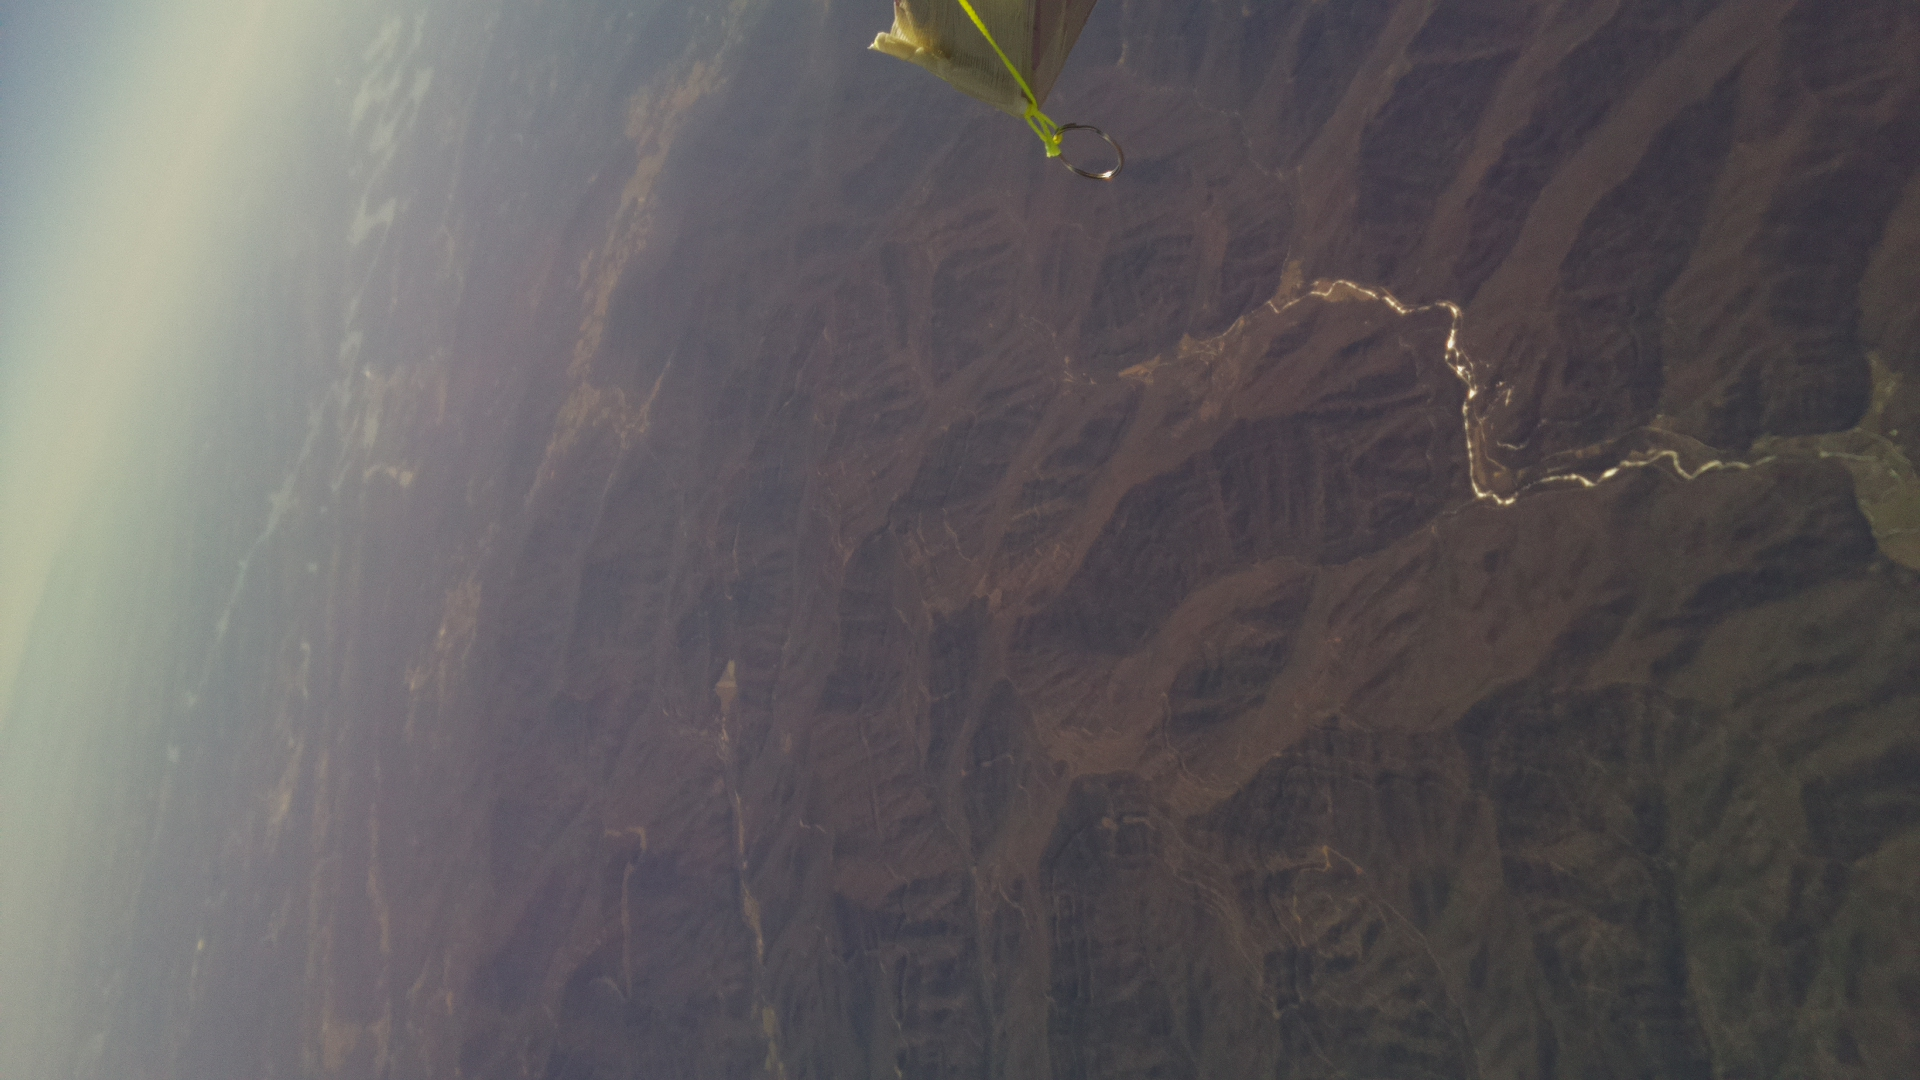
\includegraphics[width=\textwidth]{images/habpi2_4}
    \end{figure}
\end{frame}

\begin{frame}{HabPi 3 - May 13, 2017}
%Sunbright, Troop 255, CCS
\end{frame}

\begin{frame}{HabPi 4 - July 18, 2017}
%ARC Summer Institute
\end{frame}

\begin{frame}{HabPi 5 - October 7, 2017}
%Athens TN
\end{frame}

\end{document}


